\newpage
%% ML: anglictina v nazvu casti (plati pro celou praci)
%% DT: uz je nastavena cestina

\part{Webové publikační mapové platformy}
\newpage
%% ML: nazev sekce prilis obecny
%% DT: doplneno
\section{Principy mapových publikačních platforem}

\subsection{Mapy a internet}

%% ML: prvni veta, kterou jsem precetl, ma chybu v interpukci...
Lidé vytvářejí mapy po tisíce, ale již dávno je dobám, kdy bylo nutné
%% ML: mit -> vlastnit (urcite najdes lepsi vyraz)
%% DT: uchovávat
pro nahlédnutí do mapy uchovávat její fyzický otisk či originál. Problémem
takových map je jejich nákladná distribuce a omezené možnosti
obsahu. Mnohem efektivnějším způsobem jak distribuovat mapy pro
veřejnost se v dnešní době stávají webové mapové platformy. Jedna z
nejvyužívanějších \textit{Google Maps} byla spuštěna již začátkem
roku 2005 \cite{google_history}.  Obecně se mapové platformy dělí na
dvě skupiny: statické a interaktivní.

\textbf{Statické mapové platformy} nejsou z důvodu jejich úzkého
zaměření dnes již tolik běžné, avšak tvorba jejich obsahu je oproti
mapám interaktivním velice snadná. V podstatě se jedná pouze o mapový obraz vložený do webového rozhraní mapové platformy, přičemž jeho obsah je pevný a neměnný. Publikované mapové obrazy se dají vytvořit
%% ML: pomocí, "přímo" přebývá
%% ML: "scan" nezní jako slovo zapadajici do ceske vety
%% DT: skenování je lepsi
pomocí specializovaných kartografických programů, nebo skenováním
již existujících map. Takto vytvořené podklady jsou na webu velice
snadno distribuovatelné a kladou výrazně menší nároky na výpočetní
techniku.

Jak již název napovídá \textbf{interaktivní mapové platformy} jsou
takové platformy, u kterých má možnost uživatel měnit jejich
obsah. Nejčastěji se jedná o výběr podkladové mapy, filtraci mapových
prvků, přibližování a oddalování. Zjednodušeně řečeno se jedná o
interakci uživatele s webovým rozhraním dané aplikace, která dle
uživatelem kladených příkazů opakovaně aktualizuje svůj
obsah\cite{web_mapping}. Tato zkutečnost dělá z interaktivních map
velice účinný nástroj. Na druhou stranu je nutné říci, že výroba a
distribuce map pro takové platformy je o poznání složitější.

\newpage
\subsection{Fungování interaktivních mapových platforem}
\label{sssec:fungovani-platforem}

%% ML: navrhuji vynechat ``hlavne'', chybi tam porovnani s necim
%% DT: vetu jsem preformuloval
V dnešní době se v očích uživatelů těší velkému zájmu oproti statickým mapovým platformám právě mapové platformy interaktivní. Proto se jimi tato podkapitola bude
%% ML: zabyvat ?
%% DT: zabývat
zabývat podrobněji.

%% ML: pozor na dlouhe vety, souveti na jeden odstavec. Prvni cast
%% vety muze byt samostatna.
%% DT: opraveno
Interaktivních mapových platforem existuje velké množství. Jejich
základní princip fungování je však ve většině případů stejný a jednotlivé 
platformy se liší pouze svými možnostmi, obsahem a využitím.

\begin{figure}[h!]
	\centering
	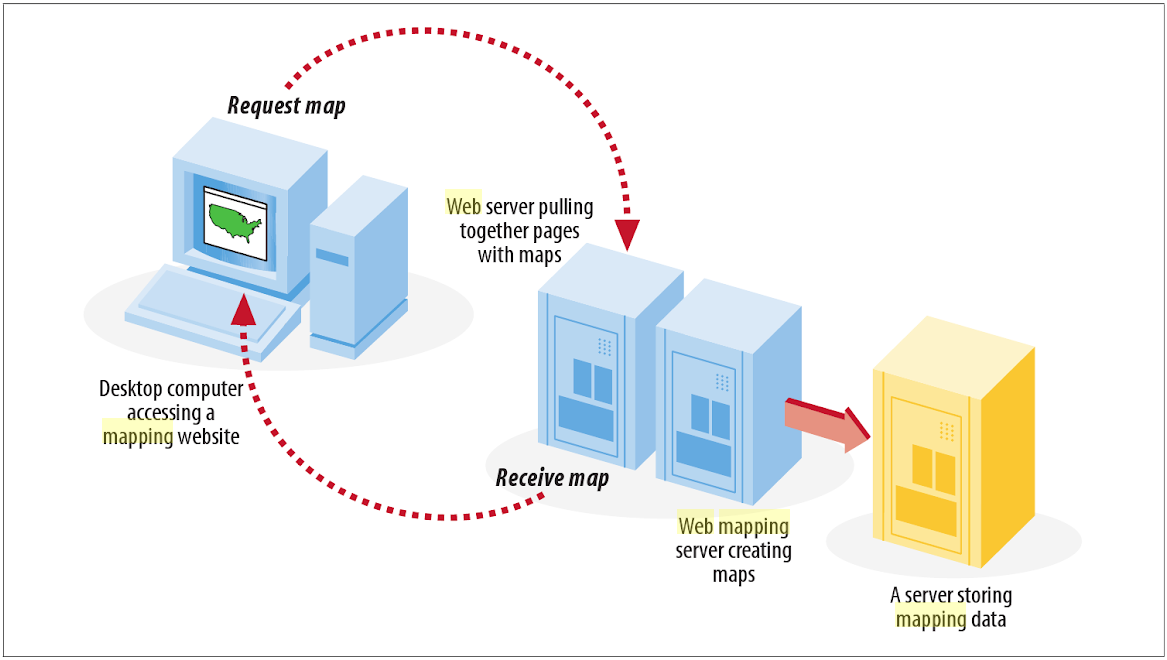
\includegraphics[width=1\textwidth]{../img/map-web-diagram.png}
%% ML: serverové části webové aplikace?
%% DT: vetu jsem preformuloval
	\caption{Diagram znázorňující základní části interaktivních mapových platforem a jejich interakci s uživatelem: \cite{web_mapping}}
	\label{fig:WPS_class_diagram}
\end{figure}

Na Obrázku 1 je znázorněn jednoduchý diagram, který popisuje fungování
interaktivní webové aplikace a jejích základních komponentů. Jedná především o tyto části:

\textit{Koncové zařízení} označované také jako webový klient,
využívající počítač, tablet, nebo mobilní telefon. Výsledná rychlost webové aplikace a její přinášený požitek dnes již není limitován tolik výpočetní
rychlostí klienta, ale především rychlostí internetového
%% ML: Vetsinu nutne komunikace
%% DT: Opraveno
připojení. Většinu nutné komunikace přitom zastává webový prohlížeč,
který pomocí \textit{request URL} získává informace z hostujícího
serveru, na kterém je webová aplikace reálně uložena.

\textit{Webový server -} přijímá požadavky od klienta a zastává nutnou
komunikaci mezi mapovým serverem a uložištěm dat. Na webovém serveru
je uložena aplikace a na vyžádání poskytuje obsah webové aplikace
%% ML: text nech nekym jeste precist, mas tam hrubky(!), silna kava, viz nize
klientovi.

\textit{Webový mapový server -} jedná se o program, který na základně
%% ML ta veta zni divne, zkus preformulovat
%% DT: změněno 
požadavků poslaných od webového klienta vytváří mapové kompozice. Data použitá mapovým serverem jsou v uložišti, do kterého má server přístup. Vytvořený mapový obraz je posléze odeslán zpět webovému klientovi. Mapových serverů existuje
%% ML: pridej odkazy na kapitoly
%% DT: doplněno
více. Těm nejvíce používaným se bude věnováno v kapitole \ref{ssec:mapove-platformy}.

\textit{Uložiště dat -} zde jsou fyzicky uložena všechna data potřebná k
vytvoření mapové kompozice, nebo její části. Jedná se o rastrová či vektorová
%% ML: mapova -> geograficka ?
%% DT: geografická
geografická data ve vhodném formátu, která dokáže webový mapový server
zpracovat. Dále jsou zde uložena metadata, která jsou nutnou součástí
%% ML: ta posledni data moc nedava smysl
%% DT: napsel jsem ji jinak
prostorových dat. Metadata popisují geografická data v předem dané struktuře \cite{web_mapping}.

Důležitou součástí každé webové mapové aplikace je samotná komunikace
mezi jednotlivými jejími komponenty. V následujících podkapitolách
bude brán zřetel převážně na komunikaci mezi webovým klientem a
webovým mapovým serverem. Konkrétně na metody, které jsou používané
%% ML: dalsi hrubka ...
%% ML: zkus posledni vetu preformulovat, v prvni vete mluvis o
%% protokolech, v druhe pise ``Tyto standardy''
%% DT: preformulovano a doplneno
pro získání mapového obrazu. Nejvíce používanou metodou, převážně v aplikacích s otevřeným kódem (viz. kapitoly \ref{sssec:mapserver}, \ref{sssec:geoserver}, \ref{sssec:qgis-server}), je použití protokolů poskytovaných mezinárodní standardizační organizací \textit{Open Geospatial Consortium (OGC)}.

\subsection{Open Geospatial Consortium}
\label{sssec:ogc}

Open Geospatial Consortium (OGC) je mezinárodní nezisková organizace
zahrnující komerční, vědecké, vládní a nevýdělečné organizace, které
se zabývají vytvářením kvalitních specifikací pro prostorová
data. Tyto specifikace jsou volně dostupné pro kohokoli za účelem
zlepšení sdílení prostorových dat po celém světě \cite{oqc_web}.

OGC specifikace jsou technické dokumenty detailně popisující rozhraní,
nebo kódování. Tyto dokumenty jsou dále použity na straně vývojářů k
%%% ML: vyvojari vetsinou nevlastni produkty :-)
%% DT: slovo "jejich" odstraněno
tvorbě produktů. Hlavním přínosem je skutečnost, že dva nezávisle
%% ML: standart -> standard (opakuje se v textu pravidelne)
%% DT: opaveno
vyvíjené programy používající OGC standardy by měly být vzájemně
kompatibilní \cite{oqc_web}. Celkem se jedná o více než 50
specifikací. Vzhledem k zaměření implementačního rámce této práce (viz. kapitoly \ref{sssec:initialization}, \ref{sssec:time-filtration}), budou konkrétněji popsány pouze následující:

\newpage
\begin{itemize}
\item\textit{Web Map Services (WMS)} - WMS nabízí jednoduché HTTP
  rozhraní pro posílání žádostí o georeferencovaný mapový obraz. Na
  základě WMS dotazu server odpoví odesláním rastrové mapy, která
  obsahuje požadované mapové prvky v daném výřezu (dlaždice).
	 
\item\textit{Web Map Tile Services (WTMS)} - princip fungování WMTS
  komunikace klient-server je obdobný jako u WMS. Rozdíl je však v
  tom, že v případě WMTS jsou požadované dlaždice již předem vytvořeny a uloženy
  v interní paměti serveru. Server je tedy nemusí při každém dotazu
  znovu vytvářet, což při velkém množství dotazů celý proces
  výrazně zrychlí.
\end{itemize}

\subsection{Web Map Services (WMS)}

%% ML: ten preklad mas odkud, zni priserne, vubec bych ho radeji
%% neuvadel, kdyz uz tak webova mapova sluzba
%% DT: preklad odstranen
WMS je mapová služba, která na základě poskytnutých
%% ML: s tim terminem ``mapa'' opatrne, kartografove by Ti to omlatili
%% o hlavu, tak alespon mapova kompozice.
%% ML: georeferencovana neni uplne korektni, georeference je soucasti
%% dotazu (bbox), vysledny obrazek uz referencovany neni, klient ho
%% ale umi korektne umistit, zna bbox
%% ML: standarta vetsinou visi nad hradem, knebo trenky ;-)
%% DT: georeferencovana mapa nahrazena mapovou kompozici
parametrů vytváří požadovanou mapovou kompozici. Mezinárodní standard dále
definuje \uv{mapový obraz} jako digitální vyobrazení geografických informací,
%% ML: preformulovat, produkt -> kompozici?
které je vhodné pro počítačové obrazovky a displeje. V případě mapové kompozice
%% ML: s terminem ``mapa'' bych setril, tak snad mapova kompozice?
%% ML: mapa obsahuje kartografickou omacku, tohle je pouze obrazova
%% kompozice geografickych dat, nic vic
%% DT: mapa opravena na mapovou kompozici
jako takové se tedy nejedná o data, ale o jejich produkt. Mapové kompozice 
%% ML: jsou poskytovány mapovych serverem v beznych obrazovych formatech...
%% DT: opraveno
jsou poskytovány mapovým serverem v běžných obrazových formátech, jako
např. PNG, GIF, nebo JPEG. Méně často se také jedná o vektorovou
grafiku ve formátech SVG, nebo WebCGM \cite{oqc_wms}.

Popisovaný standard definuje několik operací, každou s odlišným
%% ML: vraci vs. davaji
%% DT: opraveno
výstupem. Tyto operace vrací uživateli informace o
%% ML: myslis automobilovy servis? ;-) sluzbe!
samotné službě, nebo poskytují mapu či informace o zobrazovaných
mapových prvcích.

\begin{itemize}

%% ML: obecne poskytuje metadata
\item\textit{GetCapabilities} - operace vrací dokument obsahující popis 
  dat ve formátu XML.
  %% ML: souradnice -> rozsah v podporovanych souradnicovych systemech?
  %% DT: ok
  Pomocí GetCapabilities lze zjistit počet vrstev, jejich
  rozsah v podporovaných souřadnicových systémech atd.
	
\item\textit{GetMap} - jedná se o nejdůležitější operaci, protože
  %% ML: lepsi nez mapa
  jejím výsledkem je samotný mapový obraz. K jeho
  získání je potřeba poskytnout sadu parametrů, na základě kterých je
  %% ML: v?
  %% DT: mapovým
  mapovým serverem vytvořen. Těmto parametrům bude věnována následující
  %% ML: jaka
  %% DT: doplnena reference
  kapitola \ref{sssec:wms-param}.
	
\item\textit{GetFeatureInfo} - operace vrací informace o prvcích
  zobrazených na mapě.
	
\item\textit{GetLegendGraphic} - dle poskytnutých parametrů vytvoří
  tato operace legendu, kterou server vrátí jako obraz ve zvoleném
  formátu.
\end{itemize}

\subsection{Parametry WMS}
\label{sssec:wms-param}

Parametry obecně slouží ke specifikaci úkonu, který od mapového
serveru požadujeme. Jedná se tedy o vstupní informace na základě
kterých nám server odpoví. Parametrů je velké množství, některé jsou
používány vždy, některé jen velice ojediněle. Možnosti použití
%% ML: v textu pouzivas operace, presnejsi by byla asi ``dotaz''
parametrů se liší dle operace (requestu), kterou provádíme.

%% ML: mel bys uvest proc tak detailne rozepisujes parametry pro
%% GetMap
Níže uvedené parametry se vztahují pouze k operaci
\textbf{\textit{GetMap}}. Jsou zde uvedeny pouze nejdůležitější parametry a dále ty parametry, které se týkají implementační části práce (viz. kapitola \ref{sssec:time-filtration}). U operací jako \textit{GetCapabilities},
nebo \textit{GetFeatureInfo} může být popsaný význam parametrů odlišný.
V některých případech není možné parametr použít vůbec.

\begin{itemize}
\item\textit{VERSION} - specifikace verze WMS.
	
\item\textit{REQUEST} - výběr provedené operace (v případě požadavku o
 %% ML: mapu...
 %% DT: kompozice
  mapovou kompozici se jako \textit{REQUEST} parametr použije "GetMap").

%% ML: list -> seznam 
%% DT: seznam
\item\textit{LAYERS} - seznam oddělený čárkami obsahující názvy vrstev,
  které budou použity pro tvorbu mapy
	
\item\textit{SRS} - zkratka SRS v překladu znamená "geodetický
  referenční systém". Tímto parametrem je tedy určeno v jakém
  geodetickém referenčním systému jsou poskytnuté parametry
  např. BBOX.

%% ML: veta neda moc smysl, jinak Ti v textu casto chybi interpunkce
%% DT: preformulovano, nechám si to nekým opravit at s tim neni problem
\item\textit{BBOX} - jedná se o souřadnice výřezu, pro který je mapový obraz generován. Pro definování výřezu je třeba zadat
  %% ML: Pole -> Seznam
  %% DT: seznam
  souřadnice levého spodního a pravého horního rohu. Seznam souřadnic
  tedy parametr vypadá následovně "minX, minY, maxX, maxY".
	
\item\textit{FORMAT} - nastavení formátu výstupního souboru (mapového
  obrazu).
	
\item\textit{WIDTH} - celočíselná hodnota udávající šířku výsledné
  %% ML: mapa
  %% DT: mapová kompozice
  mapové kompozice v pixelech. Jinak řečeno se jedná o vzdálenost v pixelech 
  %% osa X
  osy X danou body \textit{BBOX} tj. vzdálenost minX a maxX. Osa Y odpovídá parametru \textit{HEIGHT}

\end{itemize}

Mezi další méně používané parametry patří např. \textit{EXCEPTIONS}, \textit{STYLES}, \textit{FORMAT}, \textit{ELEVATION}, \textit{BGCOLOR}, \textit{TRANSPARENT}, \textit{TIME} (jeho použití se liší viz. kapitoly \ref{sssec:mapserver}, \ref{sssec:geoserver}) \cite{oqc_wms}.

Výše uvedené parametry lze rozdělit na dvě části a to povinné a
nepovinné viz. tabulka:

\bigskip
\begin{table}[h!]
	\catcode`\-=12
	\centering
	\begin{tabular}{|c|c|}
		\hline
		parametr & povinný \\ \hline
		\hline
		VERSION & ano \\ \hline
		REQUEST & ano \\ \hline
		STYLES & ano \\ \hline
		SRS & ano \\ \hline
		BBOX & ano \\ \hline
		WIDTH & ano \\ \hline
		HEIGHT & ano \\ \hline
		TRANSPARENT & ne \\ \hline
		EXCEPTIONS & ne \\ \hline
		TIME & ne \\ \hline
		ELEVATION & ne \\ \hline
		BGCOLOR & ne \\ \hline
\end{tabular}
	\caption{Výpis parametrů a jejich povinnost použití: \cite{oqc_wms}}
	\label{tab:WPS_ExecuteRequest}
\end{table}

\subsection{Parametr TIME}
\label{sssec:time}

S ohledem na téma této práce a kapitoly \ref{sssec:mapserver}, \ref{sssec:geoserver} je vhodné přiblížit si parametr
\textit{TIME} podrobněji a popsat způsob jeho použití a možnosti,
které nabízí.

Dle OGC je formát parametru \textit{TIME} dán normou ISO 8601:1988(E),
která rozšiřuje normu ISO 8601. Oproti té jsou přidány další
specifikace\cite{oqc_wms}:
\begin{itemize}
\item Syntax pro datové kolekce. Jejich začátek, konec a periodické
  opakování.
\item Definice speciálních znaků pro vyjádření sedmi dní v týdnu.
\item Možnost zadání data před rokem 1 našeho letopočtu a to až do
  časově vzdálených geologických období (milióny a miliardy let v
  minulosti).
\end{itemize}

Základní časový formát ISO 8601:1988(E) rozšířené normy umožňuje
specifikovat časový formát až na úroveň tisícin sekund. Ne pro každou
hodnotu je však vyžadována takováto přesnost. Proto lze formát upravit
tak, že jsou odstraněny zpřesňující číslice.

\noindent
Základní formát vypadá následovně:

\begin{verbatim}
ccyy-MM-ddThh:mm:ss.SSSZ
\end{verbatim}

\noindent
A jeho zjednodušená forma pro vyjádření hodnoty s přesností na dny:

\begin{verbatim}
ccyy-MM-dd
\end{verbatim}

\newpage
\noindent
V ukázkách časových formátů jsou použita jednotlivá označení:

\begin{itemize}
	\item cc \textit{2 číslice století}
	\item yy \textit{2 číslice rok}
	\item MM \textit{2 číslice měsíc}
	\item dd \textit{2 číslice den}
	\item hh \textit{2 číslice hodina}
	\item mm \textit{2 číslice minuta}
	\item ss \textit{2 číslice sekunda}
	\item SSS \textit{3 číslice milisekunda}
\end{itemize}

\begin{itemize}
	\item T \textit{slouží k oddělení hodnot určující den a hodnot určující čas uvnitř dne}
	\item Z \textit{slouží k definici časového pásma vztaženému ke koordinovanému světovému času UTC}
\end{itemize}

Speciální znaky pro zadávání dnů v týdnu jsou: 'MON', 'TUE', 'WED',
'THU', 'FRI', 'SAT', 'SUN'. Pravěká období se definují např: M150
\textit{150 mil. let před Kristem (období Jura)}, K18 \textit{pozdní
  Doba ledová}

\newpage
\section{Webové mapové platformy}
\label{ssec:mapove-platformy}

Mapových publikačních platforem existuje v dnešní době velké
%% ML: jsou -> byly?
%% DT: byly
množství. Mohou být přizpůsobeny účelu za kterým byly vytvořeny, nebo
%% ML: Né zni divne, zkus tu vetu preformulovat.
%% DT: opraveno
konkrétním vstupním datům se kterými pracují. Podpora pro práci s časoprostorovými daty tedy není integrovaná ve všech. Tato
skutečnost je zároveň způsobena tím, že časoprostorová data nejsou
podporována všemi mapovými servery. Právě podpora na straně webového
mapového serveru je při tvorbě mapové publikační platformy
%% ML: neeee -> nikoliv
%% DT: nikoliv
klíčová, nikoliv však nutná.
 
%% ML: Veta ``jednotlive...'' je kostrbata, nedava moc smysl, preformulovat
%% DT: spojil jsem dve vety do jedne, protoze se duplikovaly
V této kapitole jsou představeny konkrétní webové mapové servery,
%% ML: posledni veta, tez preformulovat
%% DT: preformulovano
a dále je popsán jejich způsob podpory časoprostorových dat. Na závěr některých podkapitol je dále přidána ukázka webové mapové platformy využívající daný mapový server.

\subsection{MapServer}
\label{sssec:mapserver}

\begin{figure}[h!]
	\centering
	
\includegraphics[width=0.4\textwidth]{../img/mapserver-logo.png}
        %% popisek, zdroj
    \caption{Logo MapServer: \cite{mapserver_about}}
	\label{fig:mapserver-logo}
\end{figure}
\bigskip

MapServer je platforma s otevřeným kódem, která byla vytvořena pro
publikaci prostorových dat a interaktivních mapových aplikací. Byla
vytvořena v devadesátých letech na Minnesotské univerzitě. V té době se
%% ML: mas nekde OSGeo vysvetleno?, tak alespon poznamka pod carou zde
%% DT: doplneno
jednalo o jeden z prvních podporovaných projeků organizací OSGeo\footnote{\textit{OSGeo} je nevládní nezisková organizace s cílem  podporovat a prosazovat společný vývoj otevřených geoinformačních technologií a dat \cite{osgeo}}. Je
nutno podotknout, že MapServer není a ani nebyl navržen jako
%% ML: organizace? agenturou?
%% DT: agenturou
stoprocentní GIS systém. Důvod jeho vzniku je dán potřebou agentury
NASA, která hledala způsob jakým zprostředkovat satelitní snímky
%% ML: je napsan
%% DT: opraveno
veřejnosti. MapServer je napsán v jazyce C a podporuje všechny hlavní
operační systémy jakou jsou Windows, Linux a Mac OS X
\cite{mapserver_about}.

\bigskip
\noindent
\textbf{Podpora časových dat}

Od verze 4.4 je v MapServeru přidána podpora, která dokáže
%% odkaz na kapitolu o parametru time
%% DT: doplneno
interpretovat WMS parametr TIME (viz. kapitola \ref{sssec:time}) obsahující časovou hodnotu. MapServer
%% ML: dotazu
%% DT: opraveno
tuto hodnotu zpracuje a v dotazu vrátí odpovídající mapový obraz.

%% ML: urcite najdes lepsi slovo nez ``selektovat'' ;-)
%% DT: vybírat mapové prvky
K tomu, aby bylo možné vybírat mapové prvky jednotlivých vrstev pomocí atributu
TIME, musí každá vrstva obsahovat následující metadata
\cite{mapserver_about}:

\begin{itemize}
\item\textit{wms-timeextent} - povinná hodnota obsahující interval
  časových hodnot, které vrstva obsahuje. Tento interval lze zjistit
  pomocí operace \textit{GetCapabilities}.
\item\textit{wms-timeitem} - povinná hodnota obsahující název záznamu
  v databázi, ve kterém jsou časová data uložena.
\item\textit{wms-timedefault} - nepovinná hodnota určující implicitní
  hodnotu v případě, že časová hodnota pro daný záznam chybí.
\end{itemize}

\noindent
Záznam obsahující vrstvu s časoprostorovými daty vypadá následovně:

\begin{verbatim}
LAYER
	NAME "earthquakes"
	METADATA
	"wms_title"    "Earthquakes"
	"wms_timeextent" "2004-01-01/2004-02-01"
	"wms_timeitem" "TIME"
	"wms_timedefault" "2004-01-01 14:10:00"
	"wms_enable_request" "*"
	END
	TYPE POINT
	STATUS ON
	DATA "quakes"
	FILTER (`[TIME]`=`2004-01-01 14:10:00`)
	CLASS
	..
	END
END
\end{verbatim}

\bigskip
\noindent
\textbf{Formáty časových dat a syntaxe}

Výhodou použití MapServeru je jeho podpora dalších časových formátů,
které nejsou v normě ISO 8601:1988(E), používané pro operaci
\textit{WMS TIME}, definovány. Ke specifikování validních časových
formátů je možné pro každou vrstvu definovat \textit{wms-timeformat}

\begin{verbatim}
"wms_timeformat" "YYYY-MM-DDTHH
\end{verbatim}

%% ML: dotazu, ta veta mi nedava moc smysl, zkus preformulovat
%% DT: preformulovano
Dotaz s parametrem \textit{TIME} umožňuje přesně specifikovat
mapové prvky, které bude vytvořený mapový obraz obsahovat. Tímto způsobem je možné vybírat mapové prvky vrstvy pro specifické datum, nebo časový interval. MapServer
%% ML: s hodnoty?
%% DT: zmenena formulace vety
podporuje následující syntax (časové hodnoty jsou uvedeny ve formátu
'YYYY-MM-DD'):

\begin{itemize}
\item TIME=2004-10-12 \textit{pro jednu konkrétní hodnotu atributu.}
\item TIME=2004-10-12, 2004-10-13, 2004-10-14 \textit{pro více
    konkrétních hodnot.}
\item TIME=2004-10-12/2004-10-13 \textit{pro jeden konkrétní interval
    hodnot.}
\item TIME=2004-10-12/2004-10-13, 2004-10-15/2004-10-16 \textit{pro
    sjednocení více intervalů.}
\end{itemize}

\bigskip
\noindent
\textbf{Princip podpory časoprostorových dat}

%% ML: request -> dotaz
%% DT: opraveno
Princip fungování dotazu s parametrem \textit{TIME} je velice
snadný. Po té co MapServer přijme request, převede parametr
\textit{TIME} na parametr \textit{FILTER}. Tento parametr má na vstupu
název atributu obsahujícího časové hodnoty. Atribut je uložený v metadatech
časové vrstvy\cite{mapserver_about}. Další hodnotou je pouze převedená
hodnota časového parametru. V praxi vypadá filtr následovně:

\bigskip
\begin{itemize}
%% ML: selektovani -> vyber
%% DT: výber
	\item Pro výběr mapových prvků s konkrétní hodnotou
atributu, např. \textit{2004-10-12} hodnotu pro parametr 
\textit{FILTER} převede  na \textit{`[time-item]` eq `2004-10-12`}
	\item Pro selektování mapových prvků s konkrétním intervalem
hodnot, např. \textit{2004-10-12/2004-10-13}, interval pro parametr
\textit{FILTER} převede na \textit{(`[time-item]` ge `2004-10-12`) AND
(`[time-item]` le `2004-10-13`)}
\end{itemize}

%% ML: OGR neni format... (!), cela ta veta patri spise do poznamky
%% pod carou, kdyz uz
%% DT: poznamka odstranena, v kontextu prace neni dulezita

\bigskip
\noindent \textbf{Webové mapové platformy}

Webová mapová platforma zobrazující vývoj písčité pláže \textbf{Gay
Stand Sands} (\url{http://spatial.mtri.org/stampsands/}) využívá možnost
selekce časových dat. Její zvláštností však je, že k tomu není
použit parametr \textit{TIME}. Jelikož se jedná o malé množství
časových epoch, jsou tyto epochy rozděleny do jednotlivých vrstev s pojmenováním
podle časového filtru. Při requestu na konkrétní rok se tedy z
mapového serveru vrací konkrétní vrstva. Tento způsob je zvolen z
důvodu nekonzistence rastrových dat, která byla pořizována mezi lety
1938 až 2016.

\begin{figure}[h!]  \centering
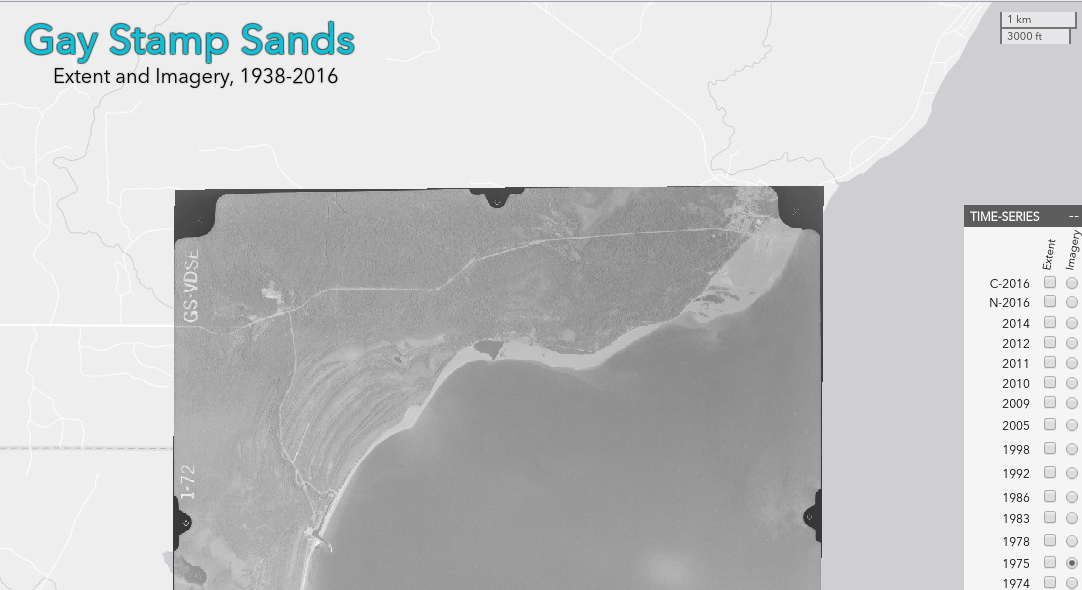
\includegraphics[width=1\textwidth]{../img/gay-sands.png}
        %% ML: screenshot nezni moc cesky, ukazka treba
        %% DT: ukazka
	\caption{Ukázka zobrazující webovou platformu Gay Stand
Sands a její uživatelské rozhraní}
	\label{fig:gay-sands}
\end{figure}

\newpage
\subsection{GeoServer}
\label{sssec:geoserver}

\begin{figure}[h!]  \centering

\includegraphics[width=0.4\textwidth]{../img/geoserver-logo.png}
	\caption{Logo GeoServer 
	\cite{geoserver-layer-edit}}
	\label{fig:geoserver-logo}
\end{figure} \bigskip

Stejně jako u MapServeru se jedná o serverový program s otevřeným
kódem. GeoServer je napsán v jazyce Java a umožňuje, na základě
otevřených standardů poskytovaných organizací OGC (viz. kapitola \ref{sssec:ogc}), sdílet a upravovat
%% ML: opravdu vsech?, co je hlavni?
%% DT: zaver vety odstranen
geografická data.

GeoServer vznikl v roce 2001 v neziskovém technologickém inkubátoru
\textit{The Open Planning Project} ve městě New York. V době vzniku bylo
hlavním cílem vytvoření sady nástrojů, které umožní větší vládní
průhlednost. Jako první nástroj vznikl právě GeoServer. Pomocí něj
mohla být veřejnost lépe zapojena do vládních záležitostí, především
územního plánování.

\begin{figure}[h!]  \centering
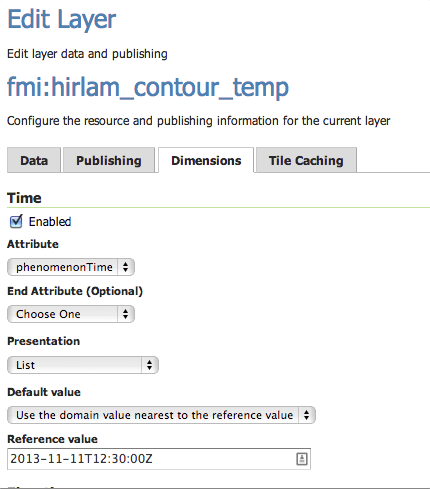
\includegraphics[width=0.6\textwidth]{../img/geoserver-layer-edit.png}
%% ML: popisky bezne zacinaji na velke pismeno\\
%% DT: vsude opraveno
	\caption{Záložka konfigurace časové vrstvy na GeoServeru
\cite{geoserver-layer-edit}}
	\label{fig:geoserver-layer-edit}
\end{figure}

\bigskip
\noindent

\textbf{Podpora časových dat}

Podpora časoprostorových dat na straně GeoServeru je velmi podobná té v
MapServeru. GeoServer podporuje v operaci \textit{GetMap} atribut
\textit{TIME}. Pro jeho použití je nutné mít správně nastavenou
vrstvu, která časová data obsahuje.

Nejjednodušším způsobem nastavení vrstvy je využití webového rozhraní
%% ML: nemel bys pouzivat cisla obrazku ``na pevno'', ale jako
%% dymamicky odkaz, navic bude potom v PDF i proklik, to se mozna tyka
%% i ostatnich obrazku (?)
%% DT: vsude dodelano
pro Geo\-Server viz. obrázek \ref{fig:geoserver-layer-edit}. V záložce \textit{Dimensions} je
nutné nastavení. V případě nastavení časové vrstvy je potřeba nejprve
zaškrtnout políčko \textit{Time Enabled}. Další nastavení je
následující \cite{geoserver-layer-edit}:

\begin{itemize}
	\item \textit{Attribute} - zde je nutné vybrat atribut, který
obsahuje časovou složku. Na základě něj jsou zjištěny časové
hodnoty. Volba atributu je možná pouze pro vektorové vrstvy.
	\item \textit{End Attribute} - jedná se o nepovinné
pole. Pomocí \textit{End Attribute} je nastavena horní hranice
intervalu hodnot, pro které je daný mapový prvek zobrazován.
	\item \textit{Presentation} - nastavení prezentace dat pro
\textit{GetCapabilities} operaci. Pokud jsou hodnoty diskrétní, tak je
možné nastavit možnost \textit{List}, \textit{interval and resolution}
pro hodnoty v intervalu s daným krokem, nebo \textit{continuous
interval} pro souvislý interval hodnot. Možnost \textit{List} je
vhodná například pro aplikace využívající animace, přičemž jeden časový
okamžik odpovídá jednomu snímku animace.
	\item \textit{Default value} - jedná se o hodnotu zastupující data, která pro zvolený atribut neobsahují žádnou časovou
hodnotu. Existuje několik možností jak \textit{Default value} zvolit:
	\begin{itemize}
		\item \textit{smallest domain value} - uloží nejnižší
hodnotu časového atributu
		\item \textit{biggest domain value} - uloží nejvyšší
hodnotu časového atributu
		\item \textit{nearest to the reference value} - uloží
hodnotu časového atributu, která je nejblíže dané referenční hodnotě
(\textit{Reference value})
%% ML: interpunkce
%% DT: opraveno
		\item \textit{reference value} - uloží danou
referenční hodnotu tak, jak je. Není brán ohled na skutečnost, zda-li je její použití vhodné.
	\end{itemize}
	\item \textit{Reference value} - pole pro zvolení referenční
hodnoty sloužící při určení \textit{Default value}.
\end{itemize}

\bigskip
\noindent \textbf{Formáty časových dat a syntaxe}

%% ML: opet request...
%% DT: opraveno
\noindent Obecná syntaxe pro dotaz s konkrétní hodnotou parametru
\textit{TIME} vypadá následovně:

\begin{verbatim} TIME=<timestring>
\end{verbatim}

Parametr \textit{TIME} je při \textit{GetMap} requestu vždy aplikován
na všechny aktuálně aktivní vrstvy definované parametrem
\textit{LAYERS}. Vrstvy bez časové složky tedy nejsou parametrem
\textit{TIME} nijak ovlivněny.

Pro zobrazení jednotlivých časových hodnot, intervalu a více hodnot je
syntaxe následující \cite{geoserver-time}:

\begin{itemize}
	\item TIME=2004-10-12 \textit{pro jednu konkrétní hodnotu
atributu.}
	\item TIME=2004-10-12,2004-10-13,2004-10-14 \textit{pro více
daných hodnot.}
	\item TIME=2004-10-12/2004-10-13 \textit{pro jeden konkrétní
interval hodnot.}
	\item TIME=2004-10-12/2004-10-13,2004-10-15/2004-10-16
\textit{pro více intervalů.}
\end{itemize}

Na první pohled je vidět, že rozdíl v syntaxi je v porovnání s MapServerem 
minimální. Mapserver však nabízí navíc možnost specifikace relativních
časových intervalů. Namísto přesné specifikace začátku a konce
intervalu je možné specifikovat začátek, nebo konec intervalu a přidat
dobu jeho trvání. Začátek či konec intervalu je zadán stejným
formátem, který je zobrazen výše. Pro hodnotu aktuálního času je možné
časovou hodnotu nahradit slovem \textit{PRESENT}.

Syntaxe pro specifikaci relativních intervalů je
následující\cite{geoserver-time}:

\begin{itemize}
	\item TIME=2002-09-01T00:00:00.0Z/P1M \textit{pro interval
hodnot pokrývající celý měsíc září 2002. Pro celý den 1. září
2002 by bylo možné použít hodnotu} P1D.
	\item TIME=P1D/2010-12-25T00:00:00.0Z \textit{pro interval
hodnot pokrývající celý den 24. prosince 2010.}
	\item TIME=PT36H/PRESENT \textit{pro časový interval 36 hodin
v minulosti od aktuálního časového okamžiku.}
\end{itemize}

\bigskip
\noindent \textbf{Webové mapové platformy}

%% ML: URL bych mohli byt proklikavaci (\url{}), to se tyka i
%% ostatnich odkazu
%% DT: opraveno vsude 
%nejsem si jist jestli je na GeoServeru \textbf{MetEye}
%% ML: nezapomen vyresit
(\url{http://www.bom.gov.au/australia/meteye}) je webová mapová platforma
zobrazující meteorologické observace a předpovědi pro celý australský
kontinent. Jedná se o interaktivní mapovou platformu vytvořenou
Australským úřadem pro meteorologii (Australian Bureaou of Metorology).

Webové rozhraní obsahuje panel s tématickými mapovými kompozicemi, 
který slouží ke specifikaci konkrétních meteorologických jevů. 
Zde lze vybrat typ předpovědi 
například vodní srážky, teplotu, sílu a směr větru atd. Mapové okno
%% ML: hrubku urcite najdes ;-)
%% DT: opravil jsem ji podle pravidla trenek na hrade
mimo standardních mapových prvků jako jsou legenda a grafické měřítko,
nabízí rovněž možnost zobrazení předpovědi počasí pro daný časový
okamžik. Toho je docíleno pomocí velice pěkně zpracované časové osy v
horní části mapového okna. Zde lze rovněž data po časových
úsecích animovat.

Rastrové vrstvy jsou filtrovány na základě parametru
\textit{TIMESTAMP}, který je vždy shodný u všech dlaždic. Vzhledem k
tomu, že pro jednotlivé předpovědi se mění pouze rastrové vrstvy, je
%% ML: hezke ceske slovo, a kdyz uz tak cache...
%% DT: nahrazeno mezipameti 
možné je na webovém serveru ukládat do mezipaměti a distribuovat ve formě dlaždic.

\begin{figure}[h!]  \centering
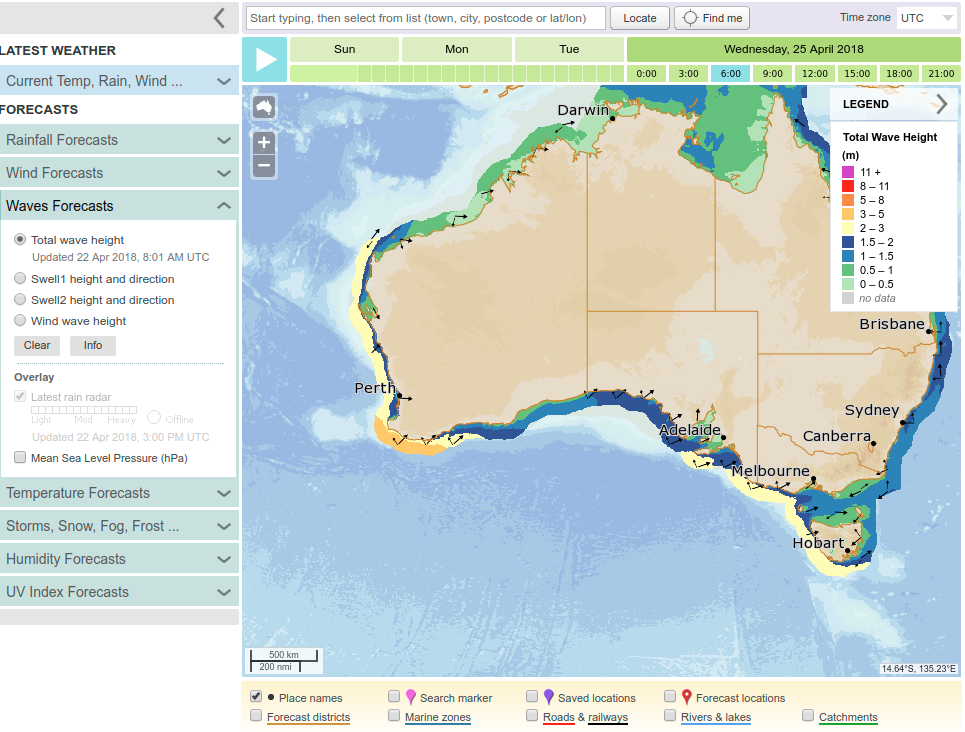
\includegraphics[width=0.67\textwidth]{../img/meteye.png}
%% ML: screenshot -> ukazka, zdroj
%% ML: doplneno
	\caption{Ukázka zobrazující webovou platformu MetEye}
	\cite{met-eye}
	\label{fig:met-eye}
\end{figure}

\textbf{Pennsylvania Cancer Atlas}
(\url{https://www.geovista.psu.edu/grants/CDC/}) je webová platforma
zobrazující výskyt rakoviny prostaty a tlustého střeva ve státě
Pensylvánie na severovýchodě USA. V tomto případě se jedná o webovou
mapovou aplikaci využívající software Adobe Flash Player, který se
spouští pomoci webového prohlížeče.

Uživatelské rozhraní nabízí tématickou mapu celého státu, která je
rozdělena na regiony. Ty jsou barevně zvýrazněny dle zastoupení
rakoviny v populaci. Pro každé období jsou dále vyhotoveny celostátní
statistiky, které jsou zobrazeny v grafech a v tabulce. Data jsou
zobrazována pro období jednoho až dvou let a pomoci jednoduchého
%% ML: selektovat
roletového menu je možné jednotlivě je selektovat nebo spustit
animaci. Pomocí panelu animace lze spustit animaci, ve které se
jednotlivá období střídají s předem daným časovým krokem. Ten dále
nabízí přeskočení na následující období a ukončení animování.

\begin{figure}[h!]  \centering
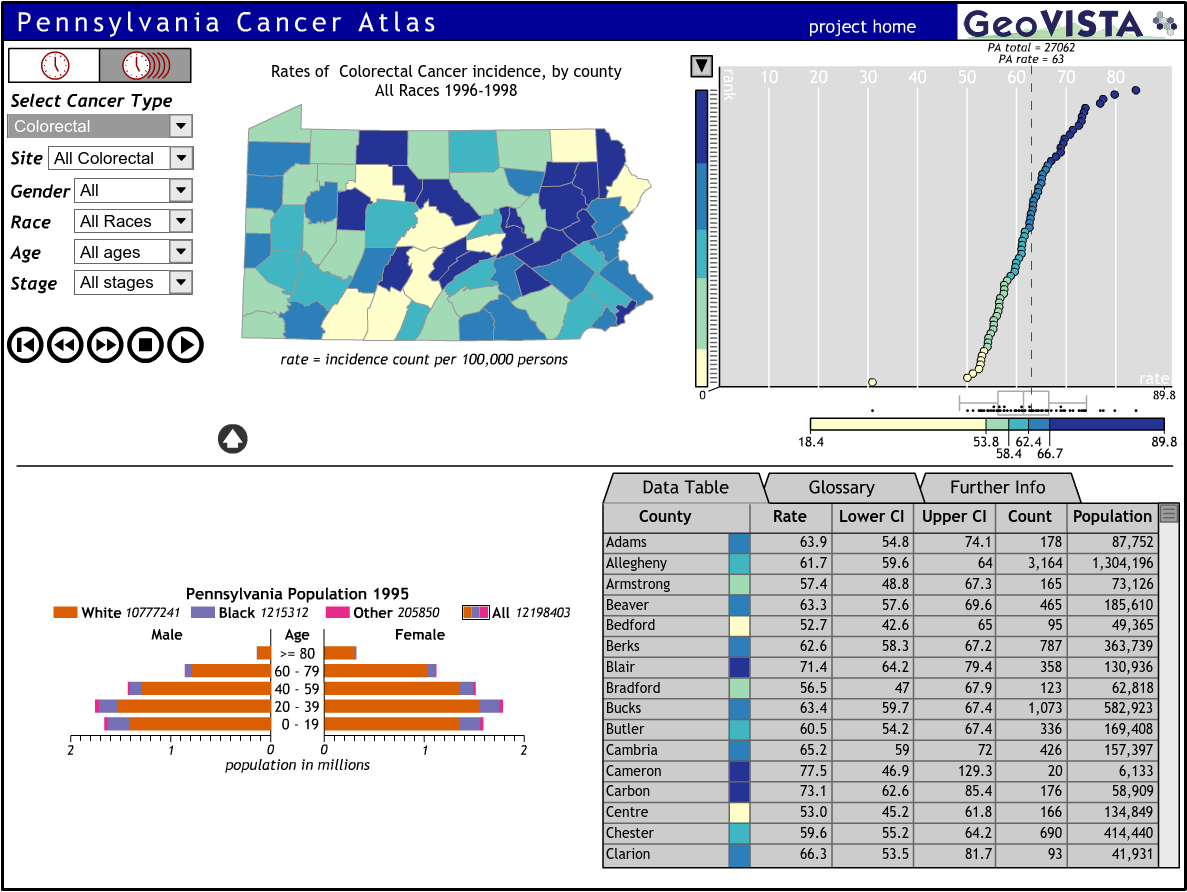
\includegraphics[width=0.8\textwidth]{../img/pennsylvania-cancer-atlas.png}
%% MK: ukazka, velke pismeno, vest zdroj
	\caption{Ukázka zobrazující webovou platformu Pennsylvania
Cancer Atlas a její uživatelské rozhraní s možností animace dle
časového období statistik}
	\cite{cancer-atlas}
	\label{fig:cancer-atlas}
\end{figure}
 
\newpage
\subsection{ArcGIS}

\begin{figure}[h!]  \centering

\includegraphics[width=0.4\textwidth]{../img/arcgis-logo.jpg}
	\caption{Logo ArcGIS}
	\cite{arcgis-logo}
	\label{fig:arcgis-logo}
\end{figure} \bigskip

ArcGIS je platforma obsahující řadu aplikací, které společně tvoří
geografický informační systém sloužící pro práci s prostorovými
daty. Nejedná se tedy o webový mapový server jako takový. ArcGIS je
%% ML: soukromy neni uplne vhodne slovo, treba proprietarni
%% DT: proprietarni
proprietární systém vytvořený firmou Esri (Environmental Systems Research
%% ML: mam pocit, ze ESRI vznikla podobne jako GRASS, nekdy na zacatku osmdesatych let
%% DT: cele jsem to preformuloval. Mam za to ye Esri vyikla takto brzy, ale ArcGIS jako takovy az pozdeji
Institute), která vznikla již v roce 1969. Nejznámějším produktem této společnosti je desktopová aplikace ArcGIS, která
se od doby svého vydání stala nejpoužívanějším komerčním softwarem na poli geografických informačních systémů \cite{arcgis-wiki}.

Pod ArcGIS patří mimo jiné aplikace pro webovou mapovou
publikaci. Jedná se o \textbf{ArcGIS Server}, \textbf{ArcGIS Online} a
\textbf{Portal for ArcGIS}.

\newpage
\subsection{ArcGIS Server}

Jedná o službu zahrnující mapování, geoprocessing, obrazové a síťové
analýzy, 3D data a možnost tvorby geografických prvků
\cite{arcgis-publishing-service}. Funkcionalita ArcGIS serveru se liší
dle balíčků, které na základě ceny omezují jeho možnosti.

\bigskip
\noindent \textbf{Podpora časových dat}
 
ArcGIS nabízí možnost práce s vrstvami obsahující časová data. K
tomu je nutné jednotlivé vrstvy ještě před jejich publikací
nastavit. V desktopové aplikaci k tomu slouží dialogové okno, které je
možné nalézt v nastavení vrstev.

\begin{figure}[h!]  \centering
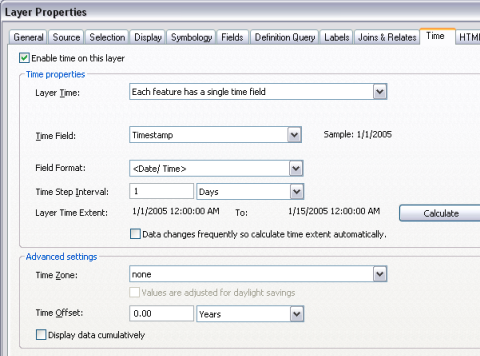
\includegraphics[width=0.8\textwidth]{../img/arcgis-layer-edit.png}
	\caption{Dialogové okno nastavení časové vrstvy v desktopové
aplikaci ArcGIS}
	\label{fig:arcgis-time-settings}
\end{figure}

K možnosti publikace je nejprve nutné zaškrtnout možnost \textit{Enable time
on this layer}. Tím bude vrstva jasně identifikována jako časová. Dále
je nutné specifikovat, jakým způsobem jsou časové hodnoty v datech
uloženy. Uloženy mohou být jako atributové pole pro vektorová data, nebo
jako rastrový katalog pro rastrová data. Nutné je rovněž nastavit
krok, jehož velikost by měla co nejlépe korespondovat s velikostí kroku, 
v jakém jsou jednotlivá data pořízena. Následující pole slouží k nastavení:

\begin{itemize}
	\item \textit{Time Properties} - v roletovém menu
\textit{Layer Time} je možnost zvolit, zda jsou data pouze v jednom
atributovém poli, nebo ve dvou. V případě dvou atributových polí 
obsahuje jedeno začátek a druhé konec časového intervalu. 
Konkrétní názvy atributů je dále nutné
zvolit z nabídky atributů pro příslušnou vrstvu. 
Poté je možné pomocí tlačítka \textit{Calculate}
vypočítat časový rozsah. Tato hodnota je posléze použita k
inicializaci časového posuvníku a rovněž k validaci časových dat. Po
výpočtu je vypsána doporučená velikost kroku časového posuvníku. Velikost
kroku lze případně změnit.
	
	\item \textit{Time Properties} - část s rozšířeným nastavením
není povinné nijak modifikovat. Obsahuje možnost specifikace časové
zóny pro použitá časová data. Takové nastavení je vhodné především pro
publikací více časových vrstev obsahující data z jiných časových
pásem. Pokud jsou jejich pásma specifikována, lze tato data snadno
kombinovat dohromady. Stejného výsledku lze také dosáhnout pomoci
nastavení časového posunu níže. V případě, že jsou některá časová data
pořízena v zemích používající změnu času na čas letní \textit{daylight
saving time}, nabízí ArcGIS tuto skutečnost u dat
specifikovat. Poslední možnost, kterou tato sekce nabízí je
\textit{Display data cumulatively} tedy kumulativní zobrazení dat. V
tom případě jsou zobrazena veškerá data mající počáteční časovou
hodnotu stejnou, nebo menší, než je hodnota aktuálně zvolená. Pokud taková data
mají nastavený konec časového intervalu je tato hodnota ignorována.
\end{itemize}

Takto nastavené vrstvy lze publikovat na ArcGIS server a pomocí
webových mapových servisů vytvářet požadované mapové obrazy. K jejich
finálnímu použití je však nutné mapový projekt publikovat na
server. Proces publikace již žádné dodatečné nastavení pro vrstvy
obsahující časová data neobsahuje, proto se mu tato kapitola věnovat
nebude.

\bigskip
\noindent \textbf{Formáty časových dat a syntaxe}

Jak již bylo upřesněno výše, časové hodnoty jsou podporovány ve třech datových
typech. Datový typ podporující datum, textový řetězec a číselná
hodnota. Pro nižší výpočetní náročnost je doporučeno maximálně využívat 
datové typy podporující datum. V případě textových řetězců je
podporováno 13 formátů a v případě číselných hodnot se jedná o 4
formáty \cite{arcgiq-data-types}.

\subsection{ArcGIS Online}

ArcGIS Online nabízí uživatelům publikování projektu přímo do cloudové
služby spravované společností ArcGIS. Nejedná se tedy o webový mapový server, ale o mapovou publikační platformu.
Způsob publikace je velice jednoduchý. V případě ArcGIS Online si není potřeba instalovat žádný software, nutné
je pouze vytvořit účet. Nabízené jsou dva hlavní typy
publikace. Jejich použití závisí na konkrétním použití aplikace. Pro
větší projekty je poté vhodná také jejich kombinace
\cite{arcgis-publishing-service}:
\begin{itemize}
	\item \textit{Feature services} - slouží především pro
publikaci atributů, mapových symbolů a dalších informací. Tyto mapové
objekty bývají často zobrazeny spolu s podkladovou mapou.
	\item \textit{Tiled map services} - jak již název napovídá,
jedná se o sadu předem generovaných mapových snímků, které jsou
serverem distribuovány ve formě mapových dlaždic. Ty mohou být pro
zvýšení výkonu aplikace drženy v mezipaměti serveru, odkud jsou přímo
dostupně přes jejich URL.
\end{itemize}

\bigskip
\noindent \textbf{Podpora časových dat} Stejně jako předchozí produkt
\textit{ArcGIS server}, tak \textit{ArcGIS online} nabízí taktéž
podporu pro práci s časoprostorovými daty. Nastavení se však liší a
vzhledem k již definovanému uživatelskému rozhraní jsou možnosti
použití rovněž omezeny na předem dané nástroje.

K tomu, aby mohla být daná vrstva označena jako časová, musí splňovat
dvě základní podmínky. Vrstva musí být typu \textit{feature layer},
\textit{map image layer}, \textit{imagery layer}, to jsou typy vrstev
podporující časové animace. Druhou podmínkou je označení konkrétní
vrstvy jako \textit{time enabled} tedy jako vrstvu podporující časová
data. Ověření podpory časových dat lze provést v \textit{map viewer} v
detailu vrstvy. Pro označení vrstvy jako časové je nutné provést kroky
popsané v podkapitole 2.4 (sekce Podpora časových dat). Pokud vrstva
splňuje obě podmínky a je označena jako viditelná zobrazí se ve spodní
části mapového prohlížeče nástroj pro správu časové vrstvy.

\begin{figure}[h!]  \centering

\includegraphics[width=0.8\textwidth]{../img/arcgis-online-time-slider.png}
	\caption{Nástroj pro správu časových vrstev}
	\label{fig:arcgis-time-slider}
\end{figure}

%vice detalneji? moznost obrazku a popisu detailniho nastaveni
casoveho nastroje Nástroj obsahuje časovou osu s posuvníky, tlačítka
pro vytvoření animace a tlačítko časového nastavení \textit{time
settings}. Po rozkliknutí tlačítka časového nastavení se zobrazí
dialogové okno, které umožňuje konfiguraci časové osy. Nastavení
dovoluje pro účely animace vrstvy změnit dobu trvání jednoho
snímku. Dále je možné omezit časovou osu jen na daný časový
interval. Implicitně je interval definován jako minimální a maximální
časová hodnota sjednocení intervalů časových hodnot pro všechny
vrstvy. V případě že není nastaveno kumulativní zobrazení dat, je
možné nastavit velikost intervalu pro který se v daný okamžik časová
data zobrazují.

Nastavení v detailu vrstvy rovněž umožňuje časový nástroj pro vrstvu
podporující časová data deaktivovat.

\newpage
\subsection{QGIS server}
\label{sssec:qgis-server}

Jedná se o mapový webový server s otevřenými daty implementující
pokročilé mapové prvky pro tvorbu tématických map. Zdrojový kód je
napsaný v programovacím jazyce C++, jsou v něm však podporované
zásuvné moduly psané jazykem Python, které umožňují rychlé a efektivní
vývoj nových komponent serveru a jeho rozšíření. V QGIS serveru jsou
implementovány standarty definované organizací OGC WMS 1.3, WFS 1.0.0
a WCS 1. Jeho vývoj byl podporován projekty Evropské unie Orchestra a
Sany a dále městem Uster ve Švýcarsku \cite{qgis-server}.

Výhoda použití QGIS serveru spočívá v použití stejné logiky jako u
desktopového QGIS. Pro vytváření map jsou použity stejné vizualizační
knihovny, které zároveň aplikují kartografická pravidla. To ve
výsledku znamená, že mapy publikované na webové publikační platformě s
použitím QGIS serveru budou vypadat stejně jako v desktopovém QGIS.

\bigskip
\noindent \textbf{Podpora časových dat}

QGIS server oproti ostatním zmíněným systémům nijak podporu pro data s
časovou složkou nepodporuje. Filtrace dat na základě parametru
\textit{TIME} tedy není možná.

Pro výše zmíněnou výhodu Qisquick platforma QGIS server používá. V
Druhé části práce bude popsáno jakým způsobem je možnost práce s
časoprostorovými daty s použitím QGIS serveru implementována.

\newpage
\subsection{Zhodnocení} V předešlých kapitolách byly popsány jednotlivé
principy a postupy práce s časoprostorovými daty pro rozdílné mapové
servery a mapové publikační platformy. Již na první pohled je zřejmé
že i přes dílčí rozdíly jsou ve všech aplikacích použity podobné
principy a pravidla.

Níže uvedená tabulka obsahuje porovnání publikačních platforem mezi 
sebou. Již na první pohled je zřejmé, že podpora časoprostorových dat ve 
volně dostupném software,
jako například MapSever a Geoserver se od sebe liší minimálně. Na 
druhou stranu licenční software v podobě ArcGIS Serveru a ArcGIS 
Online jsou od volně dostupných značně odlišné.
Vždy záleží na uživateli, zda-li preferuje otevřený zdrojový kód s širokou komunitou lidí v pozadí, nebo raději komerční software s obsáhlým uživatelským 
rozhraním. V Případě ArcGIS Online je 
použití pro mapovou publikaci nejjednodušší. Není zde nutná žádná 
instalace software, což z této platformy dělá ideální nástroj především 
pro méně zkušené uživatele.

\begin{table}[h]
	\centering
	\begin{tabular}{ | l| *6c | }
		
		  \multicolumn{1}{c}{vlastnost} & 
		  \mcrot{1}{l}{60}{MapServer} &
		  \mcrot{1}{l}{60}{GeoServer}& 
		  \mcrot{1}{l}{60}{ArcGIS Server} &   
		  \mcrot{1}{l}{60}{ArcGIS Online}  \\
		  
		  \midrule 
		  \midrule

		  možnost selekce na základě konkrétních hodnot i intervalů 
		  &  x & x & x &  \multicolumn{2}{c}{x} & \\
		  široká podpora časových formátů 
		  &  x & x & x &  \multicolumn{2}{c}{x} & \\
		  možnost nastavení časových vrstev v uživatelském
		  rozhraní 
		  &  - & x & x &  \multicolumn{2}{c}{x} & \\
		  časová hodnota mapového prvku může být interval 
		  &  - & x & x &  \multicolumn{2}{c}{x} & \\
		  nabídka časové hodnoty v případě, neexistujícího záznamu
		  &  - & x & x &  \multicolumn{2}{c}{x} & \\
		  užívající OGC standarty 
		  &  x & x & - &  \multicolumn{2}{c}{-} & \\
		  software s otevřeným kódem 
		  &  x & x & - &  \multicolumn{2}{c}{-} & \\
		  software s otevřeným zdrojovým kódem 
		  &  x & x & - &  \multicolumn{2}{c}{-} & \\
		  podpora časových pásem 
		  &  - & - & x &  \multicolumn{2}{c}{x} & \\
		  široká podpora datových typů 
		  &  - & - & x &  \multicolumn{2}{c}{x} & \\
		  bez nutnosti instalace softwaru
		  &  - & - & - &  \multicolumn{2}{c}{x} & \\
		  přímá integrace nástrojů pro práci s časoprostorovými
		  daty
		  &  - & - & - &  \multicolumn{2}{c}{x} & \\
		  
		\bottomrule
	\end{tabular}
	\caption{Výpis parametrů a jejich povinnost použití: \cite{oqc_wms}}
	\label{tab:WPS_ExecuteRequest}
\end{table}


 
